\fancyfoot[R]{\textbf{Dept. of AI\&DS, CBIT, Hyderabad}}
\chapter{INTRODUCTION}
Start Your Report Here 
\chapter{LITERATURE SURVEY}
This paper \cite{almestarihi2024measuring} is a example citation.



\chapter{METHODOLOGY}
\section{Introduction}
Brief about introduction
\section{Proposed System and System Architecture}
This is an Example Figure
\begin{figure}[H]
\centering
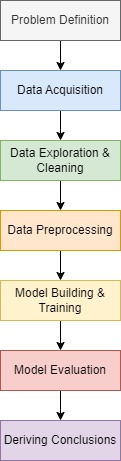
\includegraphics[width=0.2\linewidth]{methodology.jpg}
\caption{Architecture}
\label{fig:methodology}
\end{figure}
\section{Data Collection and Preprocessin}
This is an Example Table format 
\begin{table}[H]

\begin{tabular}{|l|>{\raggedright\arraybackslash}p{0.75\linewidth}|} \hline 
\textbf{Attribute} & \textbf{Description} \\
\hline
CampaignID & It is a numerical value which acts as a key.  \\
\hline
Company  & It provides the name of the company which is publishing the Ad. \\
\hline
CampaignType & It provides the medium of the campaign for example either using Email, Facebook etc.  \\
\hline
Target Audience  & This attribute consists of both the age group and the gender of the target audience. \\
\hline
Duration  & It is given in Number of Days.  \\
\hline
Channel Used  & This shows the Advertising channel used by the campaigner for example Google Ads. \\
\hline
Convertion Rate  & It shows the total number of customers purchased or converted by the total number of visitors. \\
\hline
Acquisition Cost  & It is the total money spend by an organisation in order to acquire new customers. \\
\hline
ROI  & Return on Investment.  \\
\hline
Location  & The City in which the Ad is focused on. \\
\hline
Language  & The primary language of the Ad. \\
\hline
Clicks  & Count of people going to the website by seeing the Ad. \\
\hline
Impressions  & It is a count of when each time the Ad is shown to someone. \\
\hline
Engagement Score  & It is a metric that evaluates the interaction with the Ad. \\
\hline
Customer Segment  & It broadly divides different Ads into segments such as Health and Wellness , Tech etc. \\
\hline
Date  & Date of Ad published. \\ \hline
\end{tabular}
\caption{Description of Dataset attributes}
    \label{tab:my_label}
\end{table}
\section{Model Development and Implementation}
Algorithm being utilized/Novel approach
\section{Performance Evaluation and Results}
Accuracy Comparisons with traditional and Novel Approach
\chapter{Conclusion}
\chapter{Future Scope}

%Here is a table attached :
% \begin{table}[H]
%   \centering
%        \begin{tabular}{|c|c|}
%        \hline
%        $n$ & $F_n$\\
%        \hline
%        1 & 1 \\
%        \hline
%        2 & 1 \\
%        \hline
%        3 & 2 \\
%        \hline
%        4 & 3 \\
%        \hline
%        \end{tabular}
%    \caption{Fibonacci Table}
% \end{table}
